\section{Bedienung des Programms}\raggedbottom
\label{sec:2}
Im folgenden Abschnitt soll die Bedienung der Toolbox genauer erläutert werden. Hierzu werden zunächst die Eingabeformate für die Grammatiken und Automaten beschrieben. Anschließend folgt ein Überblick über die Bedienung des Programms in der Konsole und zum Schluss wird die Bedienung der graphischen Oberfläche erläutert.
\subsection{Eingabeformat für Grammatiken}
\label{sec:2.1}
Grammatiken werden in ganz normalen Textdateien gespeichert.\\
Zu Beginn einer solchen Textdatei stehen immer die Terminal- und Nichtterminalmengen, sowie das Startsymbol. Das sieht wie folgt aus:
\lstset{
	captionpos=b,
	breaklines=true,
}
\begin{lstlisting}[frame=single, caption=Definition der Termiale und Nichtterminale]
{'a', 'b', 'c'; S, A, B; S}
\end{lstlisting}
Wie man sieht, werden die Terminale in einfache Anführungszeichen geschrieben. Ein Terminal kann eine beliebig lange Zeichenkette sein, die alle Unicode-Charaktere außer dem einzelnen Hochkomma enthalten darf. Ein Nichtterminal ist ebenfalls eine beliebig lange Zeichenkette, jedoch darf diese nur Kleinbuchstaben, Großbuchstaben, Zahlen und den Unterstrich enthalten, und darf nicht mit einer Zahl beginnen. Nach der Menge von Terminalen und der Menge von Nichtterminalen folgt jeweils ein Semikolon.\\
Anschließend folgen die Produktionen, welche so aussehen:
\begin{lstlisting}[frame=single, caption=Beispiel für eine Produktion in einer Grammatik]
A --> 'A', 'a'
\end{lstlisting}
Links steht ein Nichtterminal, dann folgt ein Pfeil und anschließend eine Liste von Terminalen und Nichtterminalen, die jeweils durch Kommata separiert sind. Hierbei ist es wichtig, dass sowohl die Terminale, als auch die Nichtterminale in einfachen Hochkommata stehen.\\
Eine vollständige Grammatik könnte zum Beispiel so aussehen:
\begin{lstlisting}[frame=single, caption=Beispiel für eine Grammatik]
{'a', 'b', 'c'; S, A, B; S}

S --> 'A', 'B'
A --> 'A', 'a'
A --> 'a'
B --> 'B', 'b'
B --> 'b'
\end{lstlisting}
\subsection{Eingabeformat von Automaten}
\label{sec:2.2}
Automaten werden ebenfalls in einfachen Textdateien gespeichert. Das Eingabeformat ist sehr ähnlich zu dem der Grammatiken.\\
Zunächst werden die Zustandsmenge, anschließend der Startzustand und zum Schluss die Endzustände des Automaten deklariert:
\begin{lstlisting}[frame=single, caption=Definition der Zustände]
{z0, z1, z2; z0; z2}
\end{lstlisting}
Der Name eines Zustandes kann beliebig lang sein und darf Kleinbuchstaben, Großbuchstaben, Zahlen und den Unterstrich enthalten, jedoch nicht mit einer Zahl anfangen. Nach der Menge der Zustände und dem Startzustand folgt jeweils ein Semikolon.\\
Nun folgen die Regeln der Übergangsfunktion:
\begin{lstlisting}[frame=single, caption=Beispiel für eine Produktion eines Automaten]
z0 --'a','b'--> z1
\end{lstlisting}
Links steht der Name des Zustands, von dem die Regel ausgeht. Es folgt ein Pfeil, in dessen Mitte die Menge an Eingabesymbolen steht, für die die Übergangsfunktion in den nächsten Zustand geht. Dieser befindet sich rechts des Pfeils befindet. Die Eingabesymbole können beliebig lang sein und sich aus allen Unicode-Charakteren, außer dem einzelnen Hochkomma, zusammensetzen und müssen selbst zwischen zwei einzelnen Hochkommata stehen.\\
Hier ist ein Beispiel für einen vollständigen Automaten:
\begin{lstlisting}[frame=single, caption=Beispiel für einen Automaten]
{z0, z1, z2; z0; z2}

z0 --'a'--> z1
z1 --'a'--> z1
z1 --'b'--> z2
z2 --'b'--> z2
\end{lstlisting}
Der daraus resultierende Automat sieht so aus:
\begin{figure}[H]
	\centering
	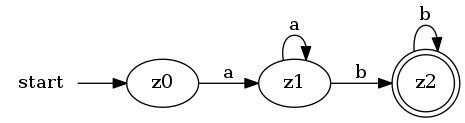
\includegraphics[width=0.75\textwidth]{bilder/beispiel_automat2.png}
	\caption{Beispiel für einen Automaten}
	\label{fig:pic2}
\end{figure}
\newpage
\subsection{Bedienung des Programms in der Konsole}
\label{sec:2.3}
Nach dem Start des Programms in einem Terminal wird man so begrüßt:
\begin{figure}[H]
	\centering
	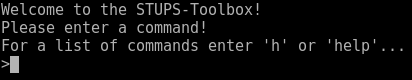
\includegraphics[width=0.75\textwidth]{bilder/konsole1.png}
	\caption{So sieht das Programm direkt nach dem Start aus}
	\label{fig:pic3}
\end{figure}
Nun hat man die Möglichkeit eine Reihe von Befehlen einzutippen, welche im folgenden aufgelistet und kurz erklärt werden.
\begin{itemize}
	\item Befehle des Hauptprogramms:
	\begin{itemize}
		\item \textit{help} oder \textit{h}:\\
		Listet alle verfügbaren Befehle mit einer kurzen Beschreibung ihrer jeweiligen Funktion auf.
		\item \textit{gui}:\\
		Öffnet die grafische Oberfläche des Programms. Die Konsole wird eingefroren, solange die grafische Oberfläche geöffnet ist und kann wieder benutzt werden, wenn sie geschlossen wird.
		\item \textit{about} oder \textit{a}:\\
		Zeigt Informationen über den aktuellen Release des Programms an.
		\item \textit{exit} oder \textit{e}:
		Beendet das Programm.
	\end{itemize}
\end{itemize}
\begin{itemize}
	\item Befehle für Grammatiken:
	\begin{itemize}
		\item \textit{load-grammar} oder \textit{lg}:\\
		Nimmt als einzigen Parameter einen Dateinamen, oder den Pfad zu einer Datei. Diese Datei sollte eine Grammatik in der in Abschnitt \hyperref[sec:2.1]{2.1} beschriebenen Form enthalten und wird dann vom Programm eingelesen und geladen.
		\item \textit{save-grammar} oder \textit{sg}:\\
		Nimmt als einzigen Parameter einen Dateinamen, oder den Pfad zu einer Datei. Die aktuell geladene Grammatik wird in dieser Datei in dem in Abschnitt \hyperref[sec:2.1]{2.1} beschriebenen Format gespeichert.
		\item \textit{print-grammar} oder \textit{pg}:\\
		Gibt die aktuell geladene Grammatik auf der Konsole aus.
		\item \textit{nullable}:\\
		Berechnet die nullable-Menge (die Menge aller Nichtterminale, die auf das leere Wort abgebildet werden können) der aktuell geladenen Grammatik und gibt sie auf der Konsole aus.
		\item \textit{first}:\\
		Berechnet die First-Menge jedes Nichtterminals der aktuell geladenen Grammatik und gibt sie auf der Konsole aus.
		\item \textit{follow}:\\
		Berechnet die Follow-Menge jedes Nichtterminals der aktuell geladenen Grammatik und gibt sie auf der Konsole aus.
	\end{itemize}
\end{itemize}
\begin{itemize}
	\item Befehle für Automaten:
	\begin{itemize}
		\item \textit{load-automaton} oder \textit{la}:\\
		Nimmt als einzigen Parameter einen Dateinamen, oder den Pfad zu einer Datei. Diese Datei sollte einen Automaten in der in Abschnitt \hyperref[sec:2.2]{2.2} beschriebenen Form enthalten und wird dann vom Programm eingelesen und geladen.
		\item \textit{save-grammar} oder \textit{sg}:\\
		Nimmt als einzigen Parameter einen Dateinamen, oder den Pfad zu einer Datei. Der aktuell geladene Automat wird in dieser Datei in dem in Abschnitt \hyperref[sec:2.2]{2.2} beschriebenen Format gespeichert.
		\item \textit{print-automaton} oder \textit{pa}:\\
		Gibt den aktuell geladenen Automaten auf der Konsole aus.
		\item \textit{graph-automaton} oder \textit{ga}:\\
		Nimmt als einzigen Parameter einen Dateinamen, oder den Pfad zu einer Datei. Der aktuell geladene Automat wird in dieser Datei im GraphViz-Format gespeichert.
		\item \textit{check-string-automaton} oder \textit{csa}:\\
		Nimmt als einzigen Parameter einen Eingabestring und prüft, ob dieser von dem aktuell geladenen Automaten akzeptiert wird. Der Eingabestring muss zwischen zwei Anführungszeichen stehen und die Eingabesymbole durch Leerzeichen getrennt sein (zum Beispiel: \textit{csa "'a a a b b c"'}).
		\item \textit{rename-states} oder \textit{rs}:\\
		Benennt die Zustände des aktuell geladenen Automaten um, so dass diese nur kurze, übersichtliche Namen haben.
		\item \textit{remove-epsilon-transitions}, oder \textit{ret}:\\
		Wandelt den aktuell geladenen Automaten in einen Automaten ohne Epsilon-Übergänge um.
		\item \textit{convert-to-dfa} oder \textit{todfa}:\\
		Wandelt den aktuell geladenen Automaten in einen DFA um. \textit{Achtung}: Der hieraus resultierende Automat hat keine vollständige Übergangsfunktion und ist somit streng genommen kein richtiger DFA. Da viele Automaten jedoch sehr unübersichtlich werden, nachdem ihre Übergangsfunktion vervollständigt wurde, habe ich mich dazu entschlossen, hierfür einen zusätzlichen Befehl hinzuzufügen.
		\item \textit{complete-automaton} oder \textit{ca}:\\
		Wandelt den aktuell geladenen Automaten in einen DFA mit einer vollständigen Übergangsfuntkion um.
		\item \textit{minimize-dfa} oder \textit{min}:\\
		Wandelt den aktuell geladenen Automaten in einen minimierten DFA um. Vor dem Umwandeln werden die Zustände des Automaten automatisch neu benannt, damit es beim Verschmelzen der Zustände nicht zu unübersichtlich wird.
	\end{itemize}
\end{itemize}
\subsection{Bedienung der grafischen Oberfläche}
\label{sec:2.4}
Durch eintippen des Befehls \textit{gui} öffnet sich ein Fenster. Hier hat man nun die Möglichkeit im \textit{Choose Plugin}-Menü eine grafische Oberfläche für Grammatiken oder Automaten auszuwählen.
\subsubsection{Grammatiken}
\label{sec:2.4.1}
Die Grammatik-GUI startet in der Bearbeitungsoberfläche. Hier wird die aktuell geladene Grammatik angezeigt und kann bearbeitet werden.
\begin{figure}[H]
	\centering
	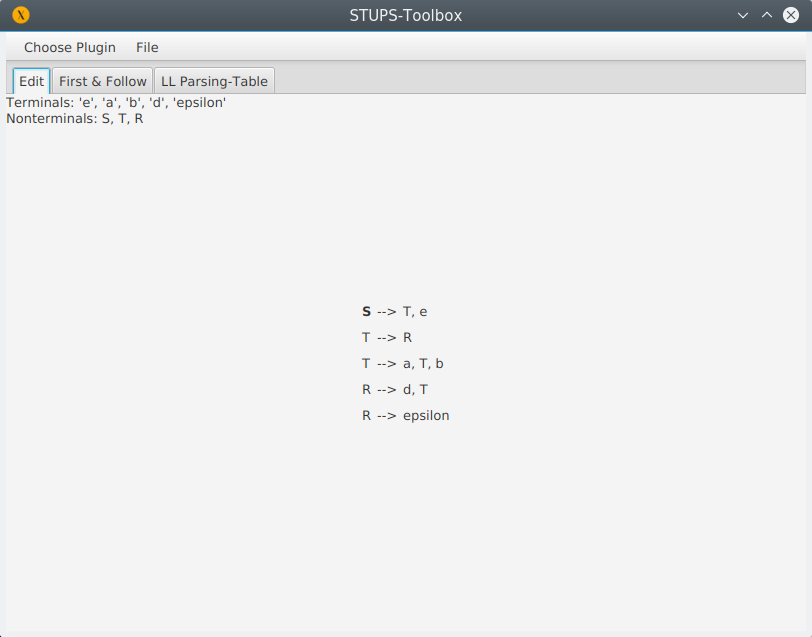
\includegraphics[width=0.75\textwidth]{bilder/gui1.png}
	\caption{Die grafische Oberfläche zeigt eine Grammatik an}
	\label{fig:pic4}
\end{figure}
\paragraph{Bedienung der Oberfläche}\ \\
Zusätzlich zum \textit{Choose Plugin}-Menü befindet sich nun noch das \textit{File}-Menü, mit welchem es möglich ist, eine neue Grammatik zu erstellen, eine Grammatik zu öffnen und die aktuelle Grammatik zu speichern.
Unter der Menüleiste sind einige Reiter zu sehen:\\
\begin{itemize}
	\item Edit:\\
	Hier wird die aktuelle Grammatik angezeigt und kann bearbeitet werden. Das Startsymbol ist fettgedruckt.
	\item First \& Follow:\\
	Hier werden nullable-, First- und Follow-Mengen der Grammatik angezeigt.
	\item LL Parsing-Table:\\
	Diese Oberfläche zeigt die LL Parser-Tabelle für die aktuelle Grammatik an. Konflikte werden rot markiert.
\end{itemize}
\paragraph{Bearbeiten einer Grammatik}\ \\
Durch Rechtsklick auf ein Nichtterminal öffnet sich ein Kontextmenü mit den Optionen \textit{Edit Symbol}, \textit{Delete Symbol} und \textit{Set as Start Symbol}.\\
Durch Auswahl von \textit{Edit Symbol} erscheint ein Textfeld anstelle des Nichtterminals, in welches man einen neuen Namen für dieses eingeben kann. Dieser Effekt wird auch durch einen Doppelklick auf das Nichtterminal erreicht.\\
Mit Klick auf \textit{Delete Symbol} wird das Nichtterminal aus der Grammatik entfernt. Dadurch werden auch alle Produktionen, bei denen es auf der linken Seite steht, entfernt.\\
\textit{Set as Start Symbol} hat zur Folge, dass das ausgewählte Nichtterminal nun das Startsymbol der Grammatik ist.\\
Auch durch Rechtsklick auf die Liste von Terminalen und Nichtterminalen öffnet sich ein Kontextmenü. Dieses hat die Einträge \textit{Edit List} und \textit{Delete Rule}.\\
\textit{Edit List} hat einen ähnlichen Effekt wie \textit{Edit Symbol}, nur dass man hier die Symbolliste bearbeiten kann. Die Symbole müssen bei der Eingabe durch Kommata getrennt sein. Auch hier ist es möglich, einfach doppelt auf die Liste zu klicken, um sie zu bearbeiten.\\
Mit \textit{Delete Rule} wird die ausgewählte Produktion aus der Grammatik entfernt. Falls in der Liste Symbole vorkommen, die in sonst keiner Produktion sind, werden diese auch aus der Grammatik entfernt.\\
Per Rechtsklick in die leere Fläche öffnet man ein Kontextmenü, dass nur den Eintrag \textit{Add Rule} enthält. Dieser öffnet ein Fenster, in welchem man eine neue Produktion erstellen kann. Hierzu müssen die linke und die rechte Seite dieser Produktion angegeben werden.
\newpage
\subsubsection{Automaten}
\label{sec:2.4.2}
Im Gegensatz zu der Grammatikoberfläche, hat die GUI für Automaten nur eine einzige Oberfläche auf der alle Funktionen vereint sind.
\begin{figure}[H]
	\centering
	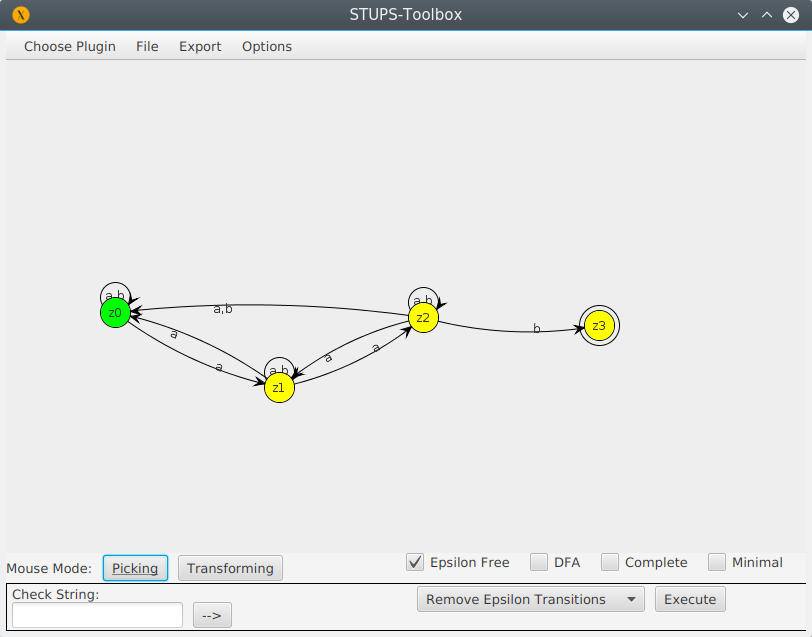
\includegraphics[width=0.75\textwidth]{bilder/gui2.png}
	\caption{Die grafische Oberfläche zeigt einen Automaten an}
	\label{fig:pic5}
\end{figure}
Auch hier finden sich neue Menüeinträge neben \textit{Choose Plugin}. Diese sind \textit{File}, womit man einen neuen Automaten erstellen, einen Automaten aus einer Datei öffnen und eine Automaten in eine Datei speichern kann, \textit{Export}, welcher es ermöglicht einen Automaten im GraphViz-Format zu speichern, und \textit{Options}, welcher zwei weitere Menüs beinhaltet, mit denen man das Layout des Übergangsgraphen und die Farben der Zustände und Produktionen anpassen kann.\\
\paragraph{Bearbeiten eines Automaten}\ \\
Im Zentrum des Fensters wird der geladene Automat angezeigt. Durch Rechtsklick auf einen Zustand, einen Produktionspfeil oder in die leere Fläche, öffnet sich ein Kontextmenü, welches, je nachdem wohin geklickt wurde, unterschiedliche Menüpunkte zum Bearbeiten des Automaten anbietet. So ist es möglich neue Zustände und Produktionen hinzuzufügen, bzw. bereits vorhandene Zustände und Produktionen zu verändern.\\
Unterhalb des Automaten sind zwei Knöpfe, mit denen man die Funktion der Maus festlegen kann. Standardmäßig ist \textit{Picking} aktiviert. In diesem Modus kann man einzelne Zustände mit der linken Maustaste auswählen und verschieben. Man kann auch mehrere Zustände auf einmal auswählen und verschieben, in dem man die linke Maustaste gedrückt hält und den Mauszeiger über die gewünschten Zustände zieht.\\
Der zweite Modus \textit{Transforming} erlaubt es den ganzen Automaten zu verschieben und zu transformieren. In dem man die linke Maustaste gedrückt hält und den Mauszeiger bewegt, kann man den Übergangsgraphen verschieben. Hält man zusätzlich noch die Strg-Taste gedrückt, kann der Graph gestreckt, bzw. gestaucht werden. Mit der Umschalt-Taste ist es möglich den Graphen zu drehen.\\
In beiden Modi lässt sich das Scrollrad der Maus benutzen um rein- und raus zu zoomen.\\
Rechts neben den beiden Knöpfen gibt es noch vier Indikatoren, die angeben, ob der angezeigte Automat frei von Epsilon-Übergängen ist, ob er ein DFA ist, ob seiner Übergangsfunktion vollständig ist, und ob er ein DFA mit einer minimalen Übergangsfunktion ist.
Im unteren Bereich des Fensters werden die geladenen Funktions-Plugins angezeigt. Hierbei wird zwischen Plugins mit eigener grafischen Oberfläche und solchen, die einfach nur eine Funktion ausführen, unterschieden. Erstere befinden sich links, letztere sind rechts in einem Dropdown-Menü aufgelistet.
\paragraph{Plugins mit grafischer Oberfläche}\ \\
\label{sec:2.4.2.1}
Momentan gibt es nur ein Plugin mit eigener grafischer Oberfläche, nämlich das \textit{Check String}-Plugin. Dieses ermöglicht es eine Eingabe für den Automaten zu simulieren. Hierzu gibt man das zu überprüfende Eingabewort in das Textfeld ein und drückt auf den Knopf mit der Beschriftung \textit{-->}. Die einzelnen Eingabesymbole müssen hierfür durch Leerzeichen getrennt sein. Wenn das Eingabewort vom Automaten akzeptiert wird, kann man durch weiteres Klicken auf \textit{-->} Schritt für Schritt sehen, wie der Automat das Wort überprüft. Mit jedem Klick auf diesen Knopf wird der nächste Zustand, oder die nächste Produktion in dem Übergangsgraphen farbig markiert. Die zur Markierung genutzte Farbe kann unter \textit{Options} --> \textit{Change colors} --> \textit{Marking color} ausgewählt werden. Standardmäßig wird rot verwendet.
\begin{figure}[H]
	\centering
	
\includegraphics[width=0.75\textwidth]{bilder/gui3.png}
	\caption{Das \textit{Check String}-Plugin mit einem Eingabewort im Textfeld}
	\label{fig:pic6}
\end{figure}
\paragraph{Plugins ohne grafische Oberfläche}\ \\
\label{sec:2.4.2.2}
Die hier verfügbaren Plugins werden unten rechts in dem Fenster in einem Dropdown-Menü aufgelistet. Um eines auszuführen, muss es in diesem Menü ausgewählt sein und der \textit{Execute}-Knopf gedrückt werden. Zur Zeit stehen folgende Plugins zur Verfügung:
\begin{itemize}
	\item Rename States:\\
	Benennt die Zustände des aktuell geladenen Automaten um, so dass diese nur noch kurze und übersichtliche Namen haben.
	\item Remove Epsilon Transitions:\\
	Wandelt den aktuell geladenen Automaten in einen ohne Epsilon-Übergänge um.
	\item Convert to DFA:\\
	Wandelt den aktuell geladenen Automaten in eine DFA um. \textit{Achtung}: Wie auch bei dem äquivalenten Konsolenbefehl gilt hier, dass nicht auf eine vollständige Übergangsfunktion geachtet wird.
	\item Complete:\\
	Wandelt den aktuell geladenen Automaten in einen DFA mit einer vollständigen Übergangsfunktion um.
	\item Minimize:\\
	Wandelt den aktuell geladenen Automaten in einen minimierten Automaten um. Wie auch bei dem äquivalenten Befehl für die Konsole werden hier vorher die Zustände umbenannt, damit die Namen nicht zu unübersichtlich werden.
\end{itemize}
\begin{figure}[H]
	\centering
	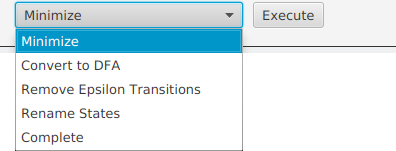
\includegraphics[width=0.75\textwidth]{bilder/gui4.png}
	\caption{Das Dropdown-Menü zeigt alle Plugins ohne grafische Oberfläche an}
	\label{fig:pic7}
\end{figure}